\chapter*{Introduction}
\addcontentsline{toc}{chapter}{Introduction}


  \section*{General context}

    \paragraph{}
    This work is rooted in the field of numerical simulation of fluid dynamics, applied to aeronautics, defense, and space industries.
    This field gathers many industrial actors (the French Direction Générale de l'Armement, ArianeGroup, Safran, Airbus, etc) as well as academics (ONERA, CERFACS, DLR, VKI, universities, etc).
    It is interested in how to simulate a fluid flow with a computer, trying to represent faithfully the physical reality.
    The various actors in this field need to be able to access certain physical quantities associated with specific phenomena and operating regimes.
    These regimes are often not feasible on our scale, due to material or financial limitations.
    Examples include the study of icing on the wing of an aircraft, which is experimentally feasible but represents an imposing budget for the aircraft manufacturer, or the study of heat transfer in an atmospheric reentry capsule, which is much more difficult to achieve experimentally.
    To overcome these limitations, numerical simulation is the best option, as it allows such a case study to be modelled by the execution of a computer program, and to obtain a large set of data that will be analysed afterwards to answer the desired questions.

    \paragraph{}
    The analysis of physics usually produces a set of equations, often partial differential equations, representing the real system that one wishes to study.
    Algorithms are then required to determine the fluid flow from these equations, in the working domain, as a function of time.
    Thus, to obtain the desired quantities, the physical system is integrated using mathematical algorithms to obtain its evolution in time.
    Often, the expected result is not the complete temporal evolution of the system, but only its equilibrium state.
    This is called a steady numerical simulation or steady computation.
    Steady computations are opposed to unsteady computations that aim to accurately describe the system's temporal evolution.

    \paragraph{}
    For all computational fluid dynamics users, the most crucial issue is to achieve a satisfying compromise between computational cost and the accuracy of the results.
    Indeed, a quick and inexpensive computation tends to be not very faithful to physics, while an accurate computation tends to use more computational resources and time.
    For steady computations, speed corresponds to getting the final steady state at a low time cost, for both computational time and the time it actually took to a user.
    It results in a compromise between methods that are expensive in terms of computational resources and take a long time but give accurate results that are close to the physical reality, and faster methods that save resources but give lesser quality results.
    A software developer working on a numerical simulation tool needs to choose methods and algorithms to obtain a compromise that is considered satisfactory.
    The final interest for a player in computational fluid dynamics is therefore to have a result that is sufficiently precise and inexpensive enough to obtain.
    An accurate result is needed to answer the questions that required the simulation.
    The search for a result that is inexpensive to obtain is motivated by questions of savings in computational cost.
    This cost is applied to the user, while he waits for the simulation to end, and to the company through the cost of computer resources, electricity, investments in more efficient machines, etc.

    \paragraph{}
    Depending on the problem to be solved, there are more or less suitable algorithms and methods.
    Performant methods were originally developed to answer the needs of the aerodynamics community.
    In the case of energetics and multiphysics problems, the methods issued from the more traditional aerodynamics are limited by the coupling  between the different physics which have their distinct characteristic times.
    Thus, the algorithms used for the numerical simulation of classical fluid dynamics are focused on the resolution of the Navier--Stokes equations, and are not necessarily the most adapted to a simulation in the field of energetics.
    The involvement of several distinct physical phenomena imposes constraints on the choice and use of algorithms.
    Consequently, it would be advisable to adapt or replace the algorithms involved in the time integration for multiphysics problems.


  \section*{Context of this thesis}

    \paragraph{}
    This thesis was conducted at ONERA, the French Aerospace Lab, in the multiphysics for energetics department.
    Although numerical simulation has been greatly developed in the aeronautical field, it has not been so well adapted to the multiphysics field, and many industrial codes are content to reuse the same algorithms.
    This is the example of the software system CEDRE, developed at ONERA by the multiphysics for energetics department \cite{ReflochCourbetMurroneEtAl2011}.
    This software system constitutes a platform grouping several solvers to integrate several physics: each solver is dedicated to its physical model.
    There is a solver for the resolution of compressible, multifluid, reactive, and turbulent flows, two solvers for the calculation of dispersed phase (drops, crystals, particles) in the Eulerian and Lagrangian approach respectively, a solver dedicated to the calculation of liquid films, a solver dedicated to radiation, etc.
    Thus, CEDRE is in fact a global platform adapted to multiphysics problems.
    Older work has been done to set up a time integration adapted to the problems solved by CEDRE \cite{Selva1998}.
    Work on time integration has led to the development of implicit integration methods for the integration of steady problems, and to the development of a GMRES method for the solution of linear systems.
    Users can choose from a panel of integration methods to obtain methods adapted to their problems.
    However, the weak coupling between solvers hampers the convergence to the steady state and the choice in integration methods is limited, compared to what can be found in the literature.
    This is at least the opinion of the actors of the CEDRE code, i.e. its developers and users, who would like more robust methods to use CEDRE on steeper problems and converge faster to save on computational costs.

    \paragraph{}
    On the research side, however, many efforts have been made in the direction of multiphysics, but have not yet left the academic framework.
    This is for example the case of \cite{WongKwokHorneEtAl2019}, who were interested in the temporal integration of coupled equations.
    They designed an integration method adapted to coupled equations, which is an evolution of a fixed point method with the addition of a step of a Newton method.
    They then compared this method to the standard fixed point method, which is more commonly used for coupled computations.
    By implementing their method on two simple coupling problems, they finally showed the value of their method compared to the more standard method.
    If this method is well fitted for their calculations, it is however only implemented for simple problems, less complex than the multiphysics problems that CEDRE wishes to solve.
    Moreover, the tests carried out are on problems on an academic scale, and not on an industrial scale.

    \paragraph{}
    At the same time, tools used in aerodynamic simulation could prove interesting for multiphysics problems.
    The Jacobian-Free Newton--Krylov method, or JFNK, is already well used in the numerical simulation of the Navier--Stokes equations.
    In \cite{ParkNourgalievMartineauEtAl2009}, a time integration mechanism is implemented around a JFNK formulation.
    A physics-based preconditioning is developed to solve the linear problem more precisely.
    This time integration is then tested on a thermally driven cavity problem.
    However, this work is only concerned with the Navier--Stokes equations and is not extended to more general energetics problems.
    Finally, it is only tested on a two-dimensional academic problem.
    In \cite{ContentOuttierCinnella2013}, it was also used on academic problems for the turbulent Navier--Stokes equations.
    The Jacobian-Free Newton--Krylov method seems to be well fitted to problems that couple multiple physics.
    It was used in \cite{Turpault2003} on applications coupling radiative transfer with hydrodynamics.
    It could prove interesting as a time integration method for CEDRE multiphysics problems.

    \paragraph{}
    \PS{This thesis was co-funded by ONERA and AID, the French agency for innovation and defence.}\footnote{\PS{Ici ?}}
    \begin{figure*}[h]
      \centering
      \begin{subfigure}[c]{0.45\textwidth}
        \centering
        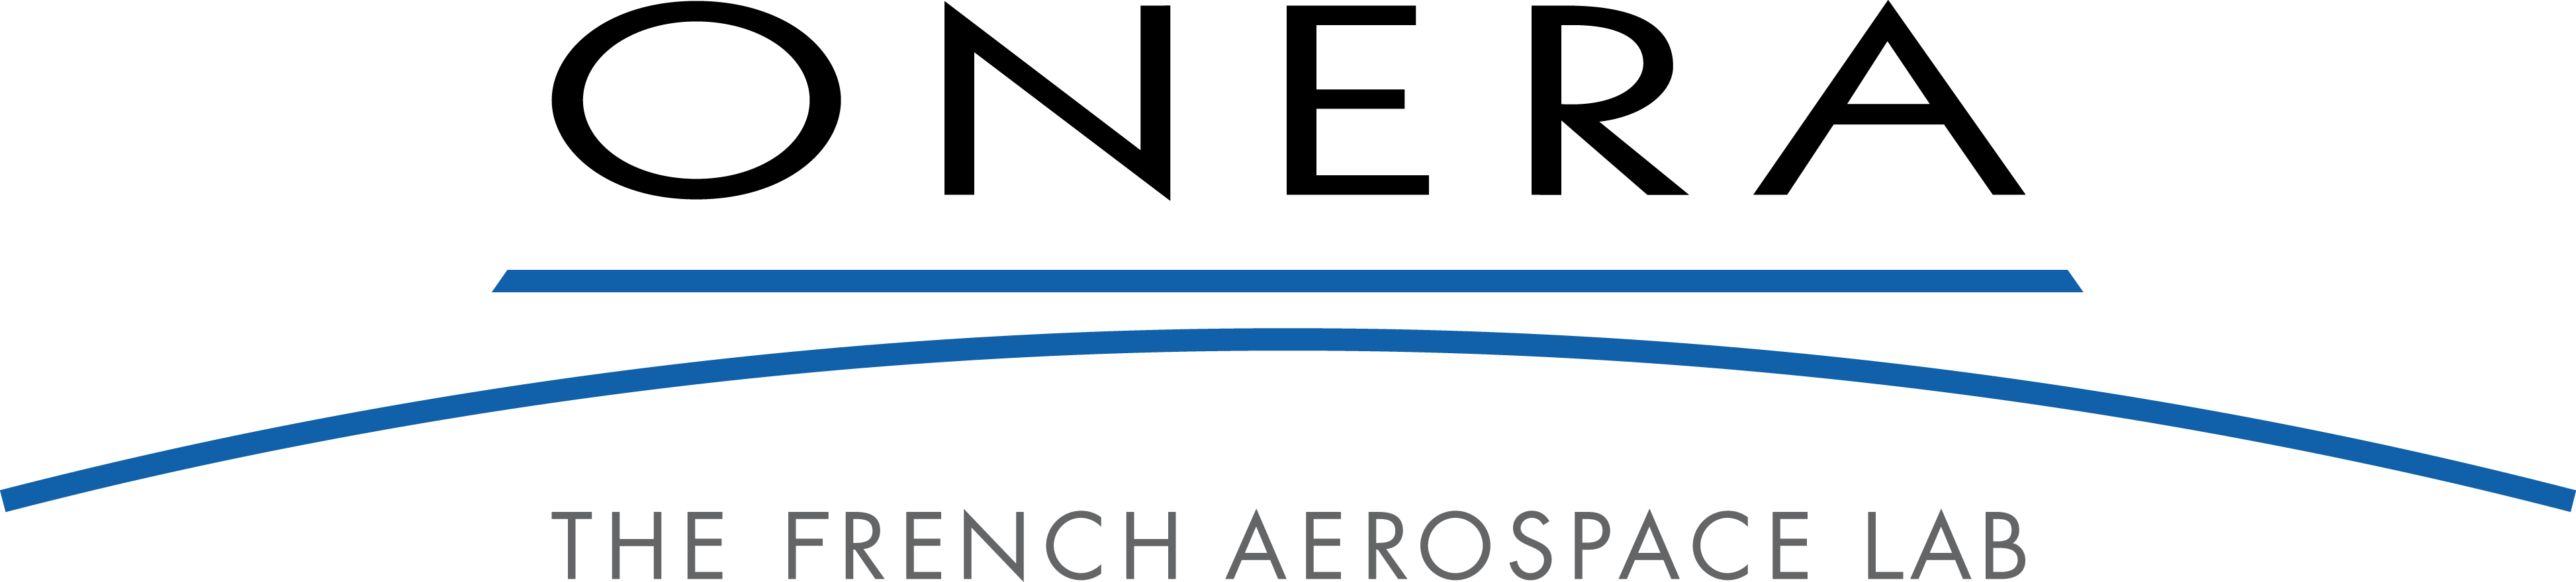
\includegraphics[width=\textwidth]{figures/logoONERA.png}
      \end{subfigure}
      \hfill
      \begin{subfigure}[c]{0.45\textwidth}
        \centering
        
\includegraphics[width=\textwidth]{figures/logoAID.jpg}
      \end{subfigure}
    \end{figure*}


  \section*{General overview and motivations}

    \paragraph{}
    It can therefore be seen that numerical methods are already available to solve computational fluid dynamics problems.
    In particular, there are already solvers capable of solving steady multiphysics problems of industrial scales.
    However, such solver use methods inherited from the aerodynamic context, that are not always adapted to handle the difficulties arising from the multiphysics properties of our problems.
    It is at least the case for our solver CEDRE.
    On the other hand, other methods developed in an academic context have shown their interest in simple multiphysics problems.
    It would now seem interesting to adapt these new methods for the resolution of multiphysics problems in an industrial code.
    This is the reason for this study.
    It consists in improving the convergence, speed and robustness of the time integration of the CEDRE platform on steady multiphysics problems by adding numerical methods not used in industrial numerical simulation.
    The aim of this work is to improve the current performances of our solver by using such more recent methods.


  \section*{Outline}

    \paragraph{}
    This document is divided into two parts.
    The first part, consisting of Chapters 1, 2, and 3, describes the work we did with the solver CEDRE, around the Jacobian-Free Newton--Krylov method.
    Some of it was presented at the 2022 Aviation Forum \cite{SeizeMatuszewskiPuigt}.
    The second part, consisting of Chapters 4 and 5, focuses on exponential time integration methods, initially investigated in CEDRE and then in another solver: JAGUAR.
    The exponential time integrator shares many ingredients with the JFNK method but is dedicated to unsteady flows.
    The novelty of the present part is the association of exponential integration and an advanced discretization technique called the Spectral Difference method.
    We plan to submit an article just after the defense on this research line.

    \paragraph{}
    The objective of Chapter 1 is to identify, from the literature, methods that we think can improve CEDRE performances, meaning speed, accuracy and robustness.
    We will introduce time integration methods and the mathematical tools we need to analyse them.
    We will go into more detail about implicit time integration methods by describing each step involved in its implementation.
    Those details will lead us from the differential equation to the algebraic solver used to solve linear systems.
    This chapter also describes what already existed in CEDRE before this thesis.
    It shows the strengths and the weaknesses of the traditional time integration methodology.
    The idea is then to work on those weaknesses by using previously identified methods.
    Indeed, we will look at the literature and choose new methods to implement that go well with what we want to keep, in place of what we want to discard.
    At this stage, we will have identified methods that we hope will improve our solver performances.

    \paragraph{}
    Chapter 2 aims to present the implementation of the new methods in CEDRE.
    To do so, we will briefly describe the structure of the solver and its different parts.
    We will then go into more detail and explain some implementation choices.
    Finally, we will justify those choices and show they are indeed valid to accomplish what set out to do.
    After this, we have a method that we need to test to see if it improves our solver performances.

    \paragraph{}
    The goal of Chapter 3 is to evaluate the robustness, accuracy and speed of the previously implemented method, and compare those performances to those of previously existing methods.
    The idea is to select representative test cases, that correspond to typical CEDRE applications.
    We will present at first simple aerodynamic test cases, and we will increase the complexity of the physical model as we go.
    For each of those test cases, we will compare the newly implemented method to the older one.
    This will justify the choices made in Chapter 1 and their implementation in Chapter 2.
    Finally, we will use the newly implemented method on an also newly implemented fluid model and show that this lead to some benefits for the solver users.

    \paragraph{}
    In Chapter 4, we will step out of the context of steady problems and extend our work to unsteady computations that use larger time steps.
    The objective of this chapter is to introduce a new category of time integration methods and give some of their characteristics.
    Then, we will show on a simple analytic test case why those new methods may be of interest to our computational fluid dynamics applications.
    We will also see that we need to use another solver to study properly those methods.

    \paragraph{}
    Chapter 5 aims to show the potential of this new class of time integration methods in our field.
    To do so, we use another solver, as was recommended in the previous chapter.
    After introducing the novelties of this other solver, we will define a set of methods we want to compare to one another, made of previously existing and newly added methods.
    Then, we describe several test cases to characterise and compare those methods.

    \paragraph{}
    Finally, we will conclude this thesis and give perspectives that can continue this work further.
